\section{Evaluierung von Verschleierungsmethoden für Penetrationstests}
\subsection{Problemstellung}
    Im Rahmen moderner Penetrationstests werden gezielt entwickelte Payloads eingesetzt, um Schwachstellen in IT-Systemen aufzudecken und die Wirksamkeit bestehender Sicherheitsmechanismen zu überprüfen. Gleichzeitig haben sich Schutzlösungen wie Endpoint Detection and Response (EDR) sowie Antivirenprogramme erheblich weiterentwickelt und sind zunehmend in der Lage, solche Payloads bereits vor ihrer Ausführung zu identifizieren und zu blockieren. Dies stellt eine Herausforderung für die realitätsnahe Simulation von Angriffsszenarien dar.\newline
    Um diese Schutzmechanismen zu umgehen und dennoch aussagekräftige Tests durchführen zu können, kommen sogenannte Verschleierungstechniken (Obfuscation) zum Einsatz. Diese zielen darauf ab, die Erkennung durch sicherheitsrelevante Systeme zu erschweren oder vollständig zu verhindern. Die Vielfalt an verfügbaren Tools und Methoden zur Obfuskation ist groß, jedoch unterscheiden sie sich teils deutlich hinsichtlich ihrer technischen Umsetzung, Benutzerfreundlichkeit und Effektivität.\newline
\subsection{Aufgabenstellung}
    Ziel dieser Arbeit ist die systematische Untersuchung und Bewertung von Verschleierungstechniken, die im Rahmen von Penetrationstests eingesetzt werden, um sicherheitsrelevante Schutzmechanismen wie Antivirus- und EDR-Systeme zu umgehen. Im Fokus steht dabei die Analyse bestehender Tools und Methoden hinsichtlich ihrer Wirksamkeit, Benutzerfreundlichkeit und Anwendbarkeit in realistischen Testumgebungen.\newline
    Zu diesem Zweck sollen zunächst geeignete Evaluierungskriterien definiert werden, anhand derer die verschiedenen Techniken vergleichend beurteilt werden können. Anschließend erfolgt die praktische Erprobung ausgewählter Obfuskationswerkzeuge in einer kontrollierten Testumgebung. Die dabei gewonnenen Erkenntnisse werden dokumentiert, analysiert und in Bezug auf ihre Relevanz für den professionellen Einsatz im Bereich der IT-Sicherheit eingeordnet.\newline
    Ein weiteres Ziel der Arbeit besteht darin, auf Basis der Evaluation mögliche Verbesserungspotenziale zu identifizieren, die als Grundlage für die Entwicklung eigener Werkzeuge oder Erweiterungen bestehender Lösungen dienen können. Die Ergebnisse dieser Untersuchung sollen somit nicht nur zur Qualitätssicherung von Penetrationstests beitragen, sondern auch Impulse für die Weiterentwicklung von Obfuskationstechniken liefern.
\subsection{Grundlagen}
Für ein klares Verständnis über das Thema sind Grundlagen unerlässlich, deshalb werden anschließend fundamentale Begriffe erklärt und ihre Bedeutung in Kontext gebracht.  
\subsubsection{Cyber Security}
Cyber-Security bezeichnet den Schutz von Computersystemen, Netzwerken und Daten vor digitalen Bedrohungen wie unautorisiertem Zugriff, Datenverlust oder Sabotage. Ziel ist es, die Vertraulichkeit, Integrität und Verfügbarkeit von Informationen sicherzustellen. Dabei umfasst Cyber-Security sowohl technische Maßnahmen (z.B. Firewalls, Verschlüsselung) als auch organisatorische Aspekte (z.B. Sicherheitsrichtlinien, Schulungen). In einer zunehmend vernetzten Welt ist Cyber-Security ein zentrales Element zur Absicherung kritischer Infrastrukturen, Unternehmenswerte und personenbezogener Daten \cite{nist800115}.
\subsubsection{Red Teaming vs. Blue Teaming}
Red Teaming und Blue Teaming sind zwei komplementäre Ansätze in der IT-Sicherheitsbewertung \cite{crowdstrike_redblue}.
\begin{itemize}
\item Das Red Team übernimmt die Rolle eines Angreifers und versucht, Schwachstellen in Systemen aktiv auszunutzen - möglichst realitätsnah und kreativ. Ziel ist es, Sicherheitslücken aufzudecken, bevor sie von echten Angreifern ausgenutzt werden.
\item Das Blue Team hingegen ist für die Verteidigung zuständig. Es überwacht Systeme, erkennt Angriffe und reagiert darauf mit geeigneten Gegenmaßnahmen.
\end{itemize}
In sogenannten \textbf{Purple Teaming}-Ansätzen arbeiten beide Teams eng zusammen, um die Effektivität von Angriffserkennung und -abwehr kontinuierlich zu verbessern.
\subsubsection{Penetration Test}
Ein Penetrationstest (kurz: Pentest) ist ein kontrollierter Sicherheitsangriff auf ein IT-System mit dem Ziel, Schwachstellen zu identifizieren und zu bewerten. Dabei simulieren Sicherheitsexperten reale Angriffsszenarien, um die Widerstandsfähigkeit von Netzwerken, Anwendungen oder Geräten zu überprüfen. Penetrationstests können manuell oder automatisiert durchgeführt werden und sind ein wichtiger Bestandteil der proaktiven IT-Sicherheitsstrategie. Sie liefern konkrete Handlungsempfehlungen zur Verbesserung der Sicherheitslage und helfen, Risiken frühzeitig zu erkennen \cite{nist800115}.
\subsubsection{Obfuscation}
Obfuscation ist eine spezielle Form der EDR/AV-Evasion, bei der der Quell- oder Maschinencode so verändert wird, dass seine Funktion schwerer zu erkennen ist – ohne dabei die eigentliche Ausführung zu beeinträchtigen. Ziel ist es, die Analyse durch Sicherheitssoftware oder forensische Tools zu erschweren. Typische Methoden sind z.B. Code Verschleierung oder Binary Verschleierung. In Penetrationstests wird Obfuscation eingesetzt, um Payloads vor der Erkennung durch Schutzsysteme zu verbergen und so realistische Angriffsszenarien zu ermöglichen \cite{you2010_obfuscation}.
\subsubsection{Portable Executable (PE)}
Das Portable-Executable-(PE)-Format ist das Standard-Dateiformat für ausführ-
bare Dateien und Bibliotheken in Windows. Es beschreibt die Struktur einer Datei, angefangen beim Header über Importtabellen bis hin zu den einzelnen Code- und Datensegmenten. Dieses Wissen ist essenziell für das Verständnis von Malware-Analyse und Penetration Testing, da Manipulationen am PE-Format – etwa durch das Injizieren zusätzlichen Codes oder durch das Umleiten von Funktionen – zentrale Angriffspfade darstellen \cite{microsoft_pe}.
\subsubsection{Shellcode}
Shellcode bezeichnet kompakten Maschinencode, der typischerweise in Assembly geschrieben und direkt vom Prozessor ausgeführt wird. Ursprünglich wurde Shellcode entwickelt, um eine Kommandozeile („Shell“) zu öffnen, hat sich aber als allgemeiner Begriff für Payloads etabliert. Im Kontext des Penetration Testing dient Shellcode häufig als exemplarischer Schadcode, mit dem Angriffe simuliert und Abwehrmechanismen überprüft werden können \cite{erickson2003}.
\subsubsection{Staged und Stageless Payloads}
Payloads lassen sich grundsätzlich in zwei Kategorien unterteilen: \textit{Staged} und \textit{Stageless}. Staged Payloads bestehen aus einem kleinen initialen Loader, der bei Ausführung zusätzlichen Code von einem externen Server nachlädt. Dies spart Speicherplatz und erlaubt flexible Angriffe, setzt aber eine funktionierende Netzwerkverbindung voraus. Stageless Payloads enthalten den gesamten Schadcode in einer Datei, sind damit größer, funktionieren jedoch unabhängig von Netzwerkbedingungen. Beide Varianten sind fester Bestandteil moderner Exploitation-Techniken und werden in Penetrationstests genutzt, um verschiedene Angriffsszenarien realistisch abzubilden \cite{metasploit_stageless}.
\subsubsection{Loader}
Ein Loader ist ein Hilfsprogramm, das eine Payload in den Speicher lädt und deren Ausführung vorbereitet \cite{metasploit_stageless, bernardinetti2023_edr}. Er übernimmt Aufgaben wie das Entschlüsseln verschleierter Payloads, das Platzieren im Arbeitsspeicher und die Initialisierung der Ausführung. Im Penetration Testing dient ein Loader dazu, Angriffe realistisch zu simulieren und Sicherheitsmechanismen wie Antiviren-Software oder EDR-Systeme zu umgehen.  
Loader werden sowohl für *staged* als auch *stageless* Payloads eingesetzt: Staged Loader laden zunächst nur einen kleinen Initialcode und rufen danach den Haupt-Payload nach, während unstaged Loader den gesamten Code direkt enthalten. Dadurch bilden Loader die zentrale Schnittstelle zwischen theoretischem Schadcode und praktischer Ausführung, z.B. über Techniken wie Process Injection .
\subsubsection{Process Injection}
Unter Process Injection versteht man das Einschleusen und Ausführen von fremdem Code im Adressraum eines bereits laufenden Prozesses \cite{mitre_t1055}. Dadurch läuft die Payload im Kontext eines legitim erscheinenden Programms, was die Erkennung erheblich erschwert. Für Penetrationstests ist diese Technik zentral, um die Leistungsfähigkeit von Antiviren- und EDR-Systemen unter realitätsnahen Bedingungen zu prüfen.
\subsubsection{Direct Syscalls}
Bei direkten Systemaufrufen (\textit{Direct Syscalls}) werden Kernel-Funktionen unmittelbar über ihre System Call Number angesprochen \cite{forshaw_projectzero}. Dieser Ansatz umgeht die Windows-API vollständig und verhindert damit, dass sicherheitskritische Bibliotheken wie \texttt{ntdll.dll} den Aufruf abfangen können. In Penetrationstests zeigt diese Methode anschaulich, wie Angreifer Abwehrmaßnahmen durch den direkten Zugriff auf Kernel-Dienste umgehen können.
\subsubsection{Indirect Syscalls}
Bei indirekten Systemaufrufen (\textit{Indirect Syscalls}) erfolgt der Zugriff auf Kernel-Funktionen nicht über die klassische API-Schnittstelle, sondern über Umwege, etwa über Zwischensprünge im Assembler-Code oder Wrapper-Funktionen \cite{forshaw_projectzero}. Diese Technik dient dazu, sicherheitsrelevante Monitoring-Mechanismen zu umgehen, die bestimmte API-Funktionen gezielt überwachen. Penetrationstester können so untersuchen, wie zuverlässig Überwachungssysteme auf indirekte Aufrufstrukturen reagieren.
\subsubsection{NTDLL Unhooking}
Viele moderne Sicherheitslösungen überwachen Prozesse, indem sie Hooks in die Windows-Systembibliothek \texttt{ntdll.dll} einfügen. Diese Bibliothek bildet die Schnittstelle zwischen der Benutzer- und der Kernel-Ebene und enthält Implementierungen zahlreicher Systemaufrufe. Beim sogenannten \textit{NTDLL Unhooking} werden die von Sicherheitssoftware eingefügten Hooks entfernt, indem die veränderten Speicherbereiche durch eine unveränderte Kopie der Bibliothek ersetzt werden. Dadurch lassen sich Systemfunktionen ungehindert aufrufen, ohne dass die Überwachung durch EDR-Systeme greift. Im Penetration Testing wird diese Technik genutzt, um den praktischen Umgang mit EDR-Umgehung zu demonstrieren \cite{bernardinetti2023_edr, volatility_edr_whitepaper}.
\newpage
\subsection{Überblick der gängingen Sicherheitsmechanismen}
\begin{table}[H]
\centering
\renewcommand{\arraystretch}{1.3}
\begin{tabularx}{\textwidth}{@{}p{4cm}X@{}}
\toprule
\textbf{Kategorie} & \textbf{Zweck und Logik} \\
\midrule
SIEM & Zentrale Sammlung, Korrelation und Analyse von Logdaten zur Erkennung sicherheitsrelevanter Ereignisse. Unterstützt bei der Identifikation von Angriffsmustern und Anomalien. \\
\addlinespace
EDR & Überwachung und Analyse von Aktivitäten auf Endgeräten zur frühzeitigen Erkennung und Reaktion auf Bedrohungen. Nutzt Verhaltensanalysen und Telemetriedaten. \\
\addlinespace
NAD & Netzwerkbasierte Anomalieerkennung durch Analyse von Traffic-Flüssen und Kommunikationsmustern. Erkennt ungewöhnliche oder verdächtige Netzwerkaktivitäten. \\
\addlinespace
Firewall & Kontrolle und Überwachung des ein- und ausgehenden Datenverkehrs. Erkennt und blockiert bekannte Angriffsmuster oder verdächtige Aktivitäten anhand von Signaturen oder Heuristiken. \\

\addlinespace
Forensik & Analyse und Aufarbeitung von Sicherheitsvorfällen. Dient der Ursachenforschung, Beweissicherung und strukturierten Reaktion auf Angriffe. \\
\addlinespace
Täuschung & Einsatz von Täuschungstechniken wie Honeypots oder Ködern zur frühzeitigen Erkennung von Angreifern. Liefert Warnsignale bei unautorisierten Zugriffen. \\
\bottomrule
\end{tabularx}
\caption{Übersicht sicherheitsrelevanter Technologien und deren Funktionslogik}
\label{tab:sicherheitstechnologien}

\end{table}
Die in Tabelle~\ref{tab:sicherheitstechnologien} dargestellten Mechanismen bilden eine mehrschichtige Sicherheitsarchitektur ab, die sowohl präventive als auch reaktive Maßnahmen umfasst. Durch die Kombination von Log-Analyse, Endgeräte-Überwachung und Netzwerk-Kontrolle entsteht ein umfassendes Abwehrsystem gegen Angriffe. Ergänzend tragen forensische Verfahren und Täuschungstechniken dazu bei, Vorfälle besser zu verstehen und Angreifer frühzeitig zu identifizieren.

\newpage
\subsection{Klassifikation von Verschleierungstechniken}
In Pentests werden verschiedene Verschleierungstechniken eingesetzt, um die Erkennung durch Sicherheitsmechanismen zu umgehen. Diese Techniken sind besonders relevant in der Post-Exploitation-Phase oder bei der Exploitation Phase, wo es von bedeutung ist unentdeckt zu bleiben. 
\subsubsection{Code Obfuscation}
Code-Obfuskation bezeichnet die gezielte Veränderung des Quellcodes, um die Lesbarkeit zu reduzieren und statische Analysen zu erschweren. Typische Methoden sind Variablen- und Funktionsumbenennung, Einfügen von Dummy-Code sowie Control-Flow-Transformationen. Moderne Ansätze nutzen KI, um Obfuskationsmuster dynamisch zu optimieren und die Widerstandsfähigkeit gegen Reverse Engineering zu erhöhen \cite{golovko2024obfuscation}.
\subsubsection{Binary Obfuscation}
Binary-Obfuskation bezeichnet die Manipulation kompilierten Codes auf Maschinenebene, um Analyse und Reverse Engineering zu erschweren. Moderne Techniken umfassen Control-Flow-Obfuskation, Instruktionssubstitution, String- und Datenverschleierung, sowie Packing mit Laufzeit-Unpacking. Fortgeschrittene Verfahren wie Virtualization-basierte Obfuskation übersetzen den Originalcode in Bytecode für eine eingebettete VM. Ergänzend werden Anti-Debugging, Anti-VM und polymorphe oder metamorphe Transformationen eingesetzt. Diese Methoden erhöhen den Analyseaufwand erheblich, können jedoch die Binärgröße und den Ressourcenverbrauch steigern \cite{vmray2024obfuscation}.
\subsubsection{Statische vs. Dynamische Techniken}
Statische Evasion umfasst Techniken, die vor der Ausführung angewendet werden, um signaturbasierte Erkennung zu umgehen. Dazu gehören Encoding, Verschlüsselung mit Laufzeit-Entschlüsselung und Packing. Ergänzend werden polymorphe und metamorphe Transformationen genutzt, um Hash-basierte Signaturen zu vermeiden \cite{case2024edr}.\\
Dynamische Evasion-Techniken wirken zur Laufzeit und zielen auf die Umgehung verhaltensbasierter Analysen. Beispiele sind On-the-Fly-Decryption, Reflective DLL Loading, Process Injection sowie direkte Systemaufrufe (Syscall Obfuscation) und dynamische API-Adressauflösung. Neuere Ansätze wie HookChain kombinieren indirekte Systemaufrufe und IAT-Hooking, um EDR-Hooks zu umgehen \cite{carvalho2024hookchain}.
\subsection{Evaluierungskriterien}
Die Bewertung von Obfuskationstechniken im Kontext von Penetrationstests erfordert klar definierte Kriterien, um deren Wirksamkeit und Praxistauglichkeit zu beurteilen. Im Folgenden werden die zentralen Evaluierungsdimensionen erläutert.
\subsubsection{Erhalt der Funktionalität}
Das primäre Kriterium ist die Sicherstellung der vollständigen Funktionsfähigkeit des Payloads nach Anwendung der Obfuskation. Jede Transformation, sei es auf Quellcode- oder Binärebene, muss gewährleisten, dass die ursprüngliche Logik unverändert bleibt und der Payload in der vorgesehenen Zielumgebung lauffähig ist.
\subsubsection{Erkennung durch AV / Multi-AV}
Ein zentrales Ziel der Obfuskation ist die Umgehung signatur- und heuristikbasierter Erkennung durch Antivirenlösungen und EDR-Systeme. Daher ist die Detektionsrate durch gängige AV-Engines ein maßgeblicher Indikator für die Effektivität der eingesetzten Technik. Eine niedrige Erkennungsquote deutet auf eine hohe Tarnwirkung hin, während eine hohe Quote auf unzureichende Verschleierung schließen lässt.
\subsubsection{Performance, Größe und Effizienz}
Neben der Tarnwirkung ist die Effizienz der Obfuskation ein wesentliches Kriterium. Techniken, die zu einer signifikanten Erhöhung der Binärgröße, längeren Ladezeiten oder erhöhtem Ressourcenverbrauch führen, können in realen Angriffsszenarien auffällig wirken oder die Ausführung behindern. Daher ist eine Balance zwischen Verschleierungsgrad und Performance sicherzustellen.
\subsection{Methodik der Evaluierung}
\subsubsection{Testumgebung und Rahmenbedingungen}
Die Evaluierung der Obfuskationstools erfolgte in einer isolierten Laborumgebung auf Basis von Virtualisierung:
\begin{itemize}
  \item \textbf{Build-/Obfuskations-Host:} Kali~Linux VM (Erzeugung der Payloads, Ausführung der Obfuskationstools). Für die Obfuskation wurden öffentliche GitHub-Repositories mit entsprechenden Tools geklont und eingesetzt, um die Payloads zu verschleiern.
  \item \textbf{Multi-Engine-Scanning:} Nutzung von Open-Source Antiviren-Scanner-Werkzeugen als Ersatz für cloudbasierte Multi-Scanner (z.\,B. VirusTotal), um Datenschutzrisiken zu vermeiden und konsistente Offlinetests zu gewährleisten. Diese Scans erfolgten auf der Windows-VM.
  \item \textbf{Zielsystem (EDR):} Windows~VM mit aktivierter Windows~Defender Antivirus/EDR (Standardkonfiguration, Signatur- und Plattformupdates aktuell zum Testzeitpunkt).
  \item \textbf{Isolierung:} Getrennte vSwitches/Netzsegmente ohne ausgehende Internetverbindungen auf dem Zielsystem; Artefakttransfer ausschließlich über freigegebene, kontrollierte Kanäle (z.\,B. isolierter Host-Only-Speicher).
  \item \textbf{Reproduzierbarkeit:} Vor jedem Durchlauf VM-Snapshots (Kali und Windows) und identische Startbedingungen.
\end{itemize}
\subsubsection{Versuchsdesign und Ablauf}
Die Messung erfolgte systematisch, um Basislinie, Obfuskationseffekt und EDR-Reaktion vergleichbar zu machen:
\begin{enumerate}
  \item \textbf{Baseline-Erzeugung:} Generierung einer nicht verschleierten Referenz-Payload (\emph{Baseline}) in der Kali-VM. Erfassung der Grundmetriken (Dateigröße und Hash z.B.).
  \item \textbf{Obfuskation:} Anwendung der zu bewertenden Tools/Techniken auf die Baseline unter definierten Parametern. Jede Tool-Konfiguration ergibt ein eigenständiges Artefakt.
  \item \textbf{Lokaler AV-Scan:} Scan der Artefakte mit Open-Source-AV-Tools auf der Windows-VM. Dokumentation von Erkennungsstatus, Engine-Treffern, Erkennungskategorien und Scan-Zeit.
  \item \textbf{Transfer \texorpdfstring{$\rightarrow$}{->} Ziel-VM:} Überführung der Artefakte auf die Windows-VM (on-write-Erkennung erfassen).
  \item \textbf{EDR-Beobachtung:} 
    \begin{enumerate}
      \item \emph{On-access/on-write:} Wird die Datei beim Kopieren/Entpacken blockiert/quarantänisiert?
      \item \emph{On-execution:} Startversuch unter kontrollierten Bedingungen (kein externes C\&C; rein lokaler, ungefährlicher Testpfad). Erfassung von Defender-Meldungen, Blockieraktion, Erkennungsname und Zeit bis zur Reaktion.
      \item \emph{Funktionalität:} Prüfen, ob der Payload seine (für den Test konzipierte, nicht-schädliche) Zielaktion erreicht (\emph{Functional Pass/Fail}).
    \end{enumerate}
  \item \textbf{Wiederholungen und Randomisierung:} Pro Tool/Parameterisierung mindestens $n \geq 3$ Wiederholungen; Reihenfolge der Tests randomisiert, um Reihenfolgeeffekte zu minimieren.
\end{enumerate}
\subsubsection{Sicherheits-, Compliance- und Gültigkeitsaspekte}
Die Tests fanden ausschließlich in einer abgeschotteten Laborumgebung statt; es wurden keine produktiven Systeme oder externen Dienste eingebunden. Die Payloads wurden so gestaltet, dass sie ausschließlich lokale, ungefährliche Testhandlungen ausführen. Ergebnisse gelten für die spezifizierte Plattform-/Konfigurationskombination, nicht notwendigerweise für andere EDR-Lösungen oder Systemstände.
\subsection{Analyse bestehender Methoden}
Der Fokus dieser Arbeit liegt auf dem Erlernen und praktischen Anwenden verschiedener Obfuskationsmethoden. Zahlreiche dieser Techniken sind in Form von Open-Source-Tools auf GitHub verfügbar, die sich hervorragend dazu eignen, deren Funktionsweise und Wirksamkeit in praxisnahen Szenarien zu untersuchen.  
Im Rahmen dieser Arbeit werden insbesondere die folgenden Werkzeuge betrachtet. Nach einer Beschreibung der Funktionsweise des Tools, werden Screenshots als Beispiel dargestellt. 

\begin{enumerate}
  \item \textbf{CTFPacker}:  
  CTFPacker ist ein Werkzeug, das primär für den Einsatz in Capture-the-Flag (CTF) Szenarien entwickelt wurde, um Antiviren- und EDR-Systeme zu umgehen. Das Tool nimmt eine Payload als Eingabe entgegen und erzeugt unter Verwendung spezifischer Flags eine Ausgabedatei (DLL oder EXE) mit den gewünschten Funktionen.
  \begin{figure}[H]
    \centering
    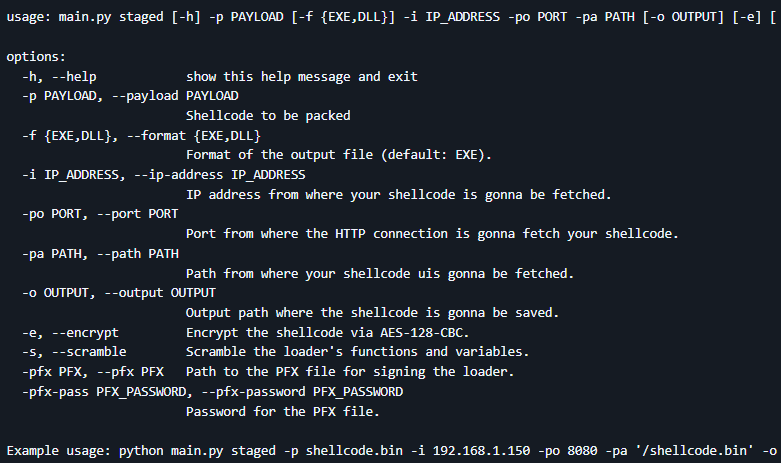
\includegraphics[width=1\textwidth]{Praxisarbeit/IMG/bilder/CTFPacker/ctfpacker1.png}
    \caption{Staged Payload Erzeugung Syntax}
    \label{Staged Payload Erzeugung Syntax}
\end{figure}
  \begin{figure}[H]
    \centering
    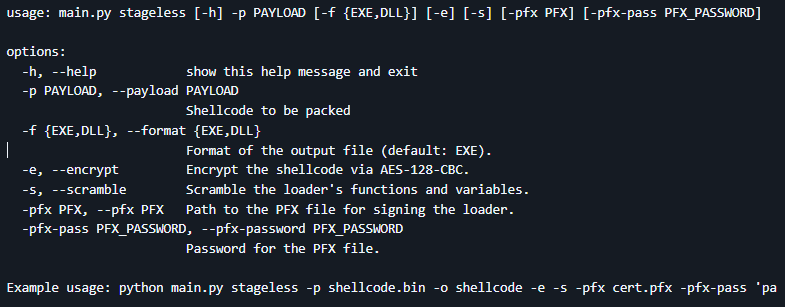
\includegraphics[width=1\textwidth]{Praxisarbeit/IMG/bilder/CTFPacker/ctfpacker2.png}
    \caption{Stageless Payload Erzeugung Syntax}
    \label{Stageless Payload Erzeugung Syntax}
\end{figure}
Die Installation gestaltete sich unkompliziert und erforderte lediglich wenige Schritte sowie das Einrichten einiger Abhängigkeiten. Verschiedene Obfuskations- und Verschlüsselungsoptionen konfiguriert werden \cite{ctfpacker}. Unter anderem gehören dazu \emph{indirekte Syscalls}, wobei es darum geht, Systemaufrufe an den Kernel nicht über die normale, direkte Bibliotheks-„Schalter“-Route auszuführen, sondern über einen Umweg, wodurch die Herkunft des Aufrufs für Überwachungstools weniger offensichtlich ist.\newline
Das Tool bietet darüber hinaus mehrere weitere, klar abgrenzbare Funktionalitäten: \emph{API-Hashing} ersetzt lesbare Funktionsnamen durch kompakte Hash-Werte zur Erkennungs Erschwerung und Größenreduktion. Eigene Implementierungen von \texttt{GetProcAddress} und \texttt{GetModuleHandle} erlauben das Auflösen von Funktions- und Moduladressen ohne die Standard-APIs sichtbar zu verwenden. Zur Reduktion von Beobachtbarkeit setzt das Projekt eine Form des \emph{NTDLL-Unhooking} mittels der Known-DLLs-Technik ein, also das Ausnutzen bereits vorhandener, als „bekannt“ registrierter DLL-Stellungen, anstatt zusätzliche Hook-Artefakte im Prozess zu hinterlassen.\newline
Für die Vertraulichkeit und Integrität von Artefakten stellt das Tool eine \emph{Custom AES-128-CBC}-Implementierung zur Verfügung, die Verschlüsselung und Entschlüsselung von Payloads in einem gängigen Blockmodus ermöglicht. Auf der Ausführungsebene wird als Injektionsvariante unter anderem die \emph{EarlyBird APC Injection} unterstützt, eine Technik, die den Startkontext von Threads ausnutzt, um Code auszuführen, ohne unmittelbar sichtbare neue Prozesse zu erzeugen. Nutzer können wählen, ob der Loader \emph{staged} arbeitet (mehrteiliger Übertragungs-/Ladeschritt) oder \emph{stageless} (voll integrierte Einzelkomponente). Schließlich bietet ein \emph{polymorpher} Modus (Aufruf mit dem \texttt{-s}-Argument) einfache Variantenbildung zur Veränderung der Binärstruktur bei wiederholter Generierung, was der Signaturbasierten Erkennung zusätzliche Hürden bereitet.\newline
Diese Funktionalitäten sind in der Gesamtheit als modulare Optionen implementiert und erlauben die flexible Konfiguration des Generierungs- und Ladeverhaltens. \cite{ctfpacker}\newline
  \item \textbf{Donut}:  
Donut ist ein äußerst leistungsfähiges Werkzeug mit einem klar umrissenen Funktionsumfang: Es konvertiert eine gegebene Payload in ein PE-Format in verschlüsselten Raw-Shellcode. Besonders vorteilhaft ist die Kombination mit beispielsweise \emph{ScareCrow}, da dieses Tool ausschließlich Shellcode als Eingabe akzeptiert \cite{donut}.
\begin{figure}[H]
    \centering
    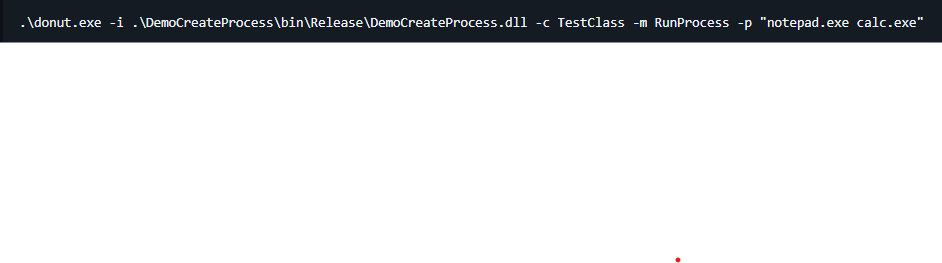
\includegraphics[width=1\textwidth]{Praxisarbeit/IMG/bilder/Donut/donut.png}
    \caption{Donut Syntax}
    \label{Donut syntax}
\end{figure}
Erweiterte Funktionalitäten von Donut lassen sich in mehrere, gut unterscheidbare Bereiche gliedern: Für unterschiedliche Eingabeformate stellt Donut jeweils spezialisierte Loader bereit — so existieren eigene Loader für \texttt{.NET}-Assemblies, für Skripte (VBScript/JScript) sowie für native PE-Dateien. Bei \texttt{.NET}-Assemblies nutzt Donut das Unmanaged CLR-Hosting, erstellt temporäre AppDomains und lädt die Assembly über die vom Hosting-API vorgesehenen Methoden, um anschließend den Entry-Point oder eine benannte Methode auszuführen. Skriptdateien werden über die Windows-Schnittstelle \texttt{IActiveScript} ausgeführt, während native Binaries durch einen eigenen In-Memory-PE-Loader betrieben werden, der typische PE-Eigenarten wie Delayed Imports oder TLS\footnote{TLS = Thread-Local Storage ist ein Mechanismus, der jedem Thread eigene, unabhängige Speicherplätze (Variablen) zur Verfügung stellt. Das bedeutet: mehrere Threads können dieselben Variablennamen benutzen, ohne sich gegenseitig zu überschreiben\cite{ms_tls_2025}} berücksichtigt. Diese Trennung nach Dateityp erlaubt eine robuste und flexible Handhabung verschiedener Payload-Formate.\newline
Zur Reduktion der Erkennbarkeit implementiert Donut mehrere, modular ausgelegte Schutzmechanismen: optionales Deaktivieren von AMSI\footnote{AMSI ist eine Windows-Schnittstelle, die Anwendungen ermöglicht, Inhalte (z. B. Skripte oder dynamisch erzeugten Code) zur Prüfung an lokal installierte Antimalware-Produkte zu übergeben. Dadurch können Defender/AV-Produkte Inhalte zur Laufzeit inspizieren und gegebenenfalls blockieren oder melden.\cite{ms_amsi_2025}} und WLDP\footnote{WLDP bezeichnet Windows-APIs und Mechanismen zur Abfrage und Durchsetzung von „Lockdown“-/Device-Guard-/Ausführungsrichtlinien (z. B. ob dynamischer/unsignierter Code ausgeführt werden darf). Entwickler und Systemkomponenten können WLDP-Funktionen nutzen, um die Ausführbarkeit von Code im Kontext der Plattform-Sicherheitsrichtlinien zu bewerten.\cite{ms_wldp_2022}} sowie ein ETW-Bypass\footnote{ETW ist das in Windows eingebaute Tracing/Logging-Framework, das Ereignisse aus Kernel- und User-Mode effizient sammelt und für Analyse, Performance-Monitoring oder Forensik bereitstellt.\cite{ms_etw_2024}} (standardmäßig auf Basis veröffentlichter Forschung), die alle darauf abzielen, dynamische Codeausführung weniger offensichtlich für Monitoring-Systeme zu machen. Ferner unterstützt das Projekt die Dekompression von Payloads im Arbeitsspeicher (z.B. über aPLib oder die Windows-API \texttt{RtlDecompressBuffer}) sowie ein bewusstes Handling der PE-Header: standardmäßig werden die Header eines geladenen Moduls im Speicher so angepasst oder durch die Header eines „Decoy“-Moduls ersetzt, dass ein einfacher Vergleich zwischen Speicherabbild und Datei-Metadaten Erkennungsheuristiken erschwert; es besteht jedoch auch die Möglichkeit, die Original-Header unverändert zu belassen, wenn der Payload diese benötigt.\newline
  \item \textbf{ScareCrow}:  
  ScareCrow zeichnet sich durch seine Vielseitigkeit aus, da es Raw-Shellcode als Eingabe akzeptiert und eine Vielzahl von Konfigurationsoptionen über Flag-Parameter bereitstellt. In den Tests traten jedoch wiederholt Kompilierungsprobleme bei der Erzeugung von DLL-Dateien auf, während die Generierung von EXE-Dateien konsistent möglich war. ScareCrow ist primär auf Side-Loading\footnote{Side-Loading bezeichnet eine Technik, bei der ein legitimer, signierter Prozess unbeabsichtigt eine manipulierte oder bösartige DLL lädt, weil Windows bei der Auflösung von Abhängigkeiten zunächst in bestimmten Verzeichnissen (z. B. im Anwendungsverzeichnis) nach der benötigten Bibliothek sucht. Angreifer platzieren ihre DLL dort, sodass die Anwendung sie anstelle der originalen Bibliothek lädt.} ausgelegt — das heißt, es erzeugt Loader, die legitime Windows-Prozesse als Träger nutzen, anstatt klassischen Code-Injection-Mechaniken zu folgen — und versucht anschließend, EDR-Hooks aus den im Prozess geladenen System-DLLs zu „flushen“, da viele EDR-Hooks beim Prozessstart gesetzt werden.
  \begin{figure}[H]
    \centering
    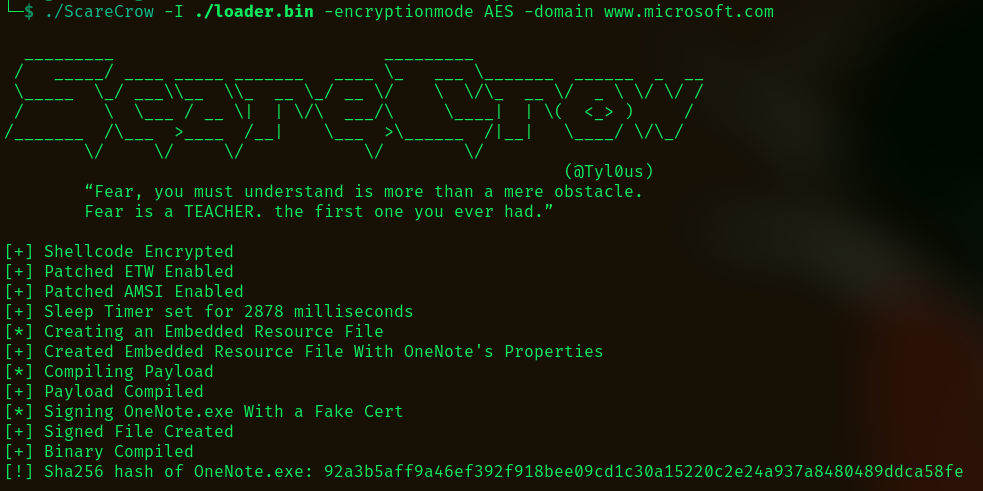
\includegraphics[width=1\textwidth]{Praxisarbeit/IMG/bilder/ScareCrow/ScareCrow.png}
    \caption{Scarecrow Beispiel Nutzung}
    \label{Scarecrow beispiel nutzung}
\end{figure}
Weitere nennenswerte Funktionen und Eigenschaften :\newline
\begin{enumerate}
    \item Modulare Loader-Struktur und mehrere Shellcode-Templates, die verschiedene Zieltypen (z. B. EXE, CPL, DLL, JS) unterstützen; die Architektur wurde in neueren Releases modularisiert.
    \item Verschlüsselungs- und Obfuskationsoptionen: wählbare Verschlüsselungsmodi (u. a. AES, RC4, LZMA) sowie Flags zur Literal-/String-Obfuskation.
    \item Mechanismus zum EDR-Bypass: Der Loader versucht, Sichtbarkeit gegenüber Laufzeit-Überwachung zu reduzieren (z. B. durch das Entfernen/Überschreiben von Hook-Artefakten in System-DLLs). Das Projekt enthält außerdem Hinweise und Materialien zur Erkennung solcher Techniken aus Verteidiger-Perspektive.
    \item Binary- und Template-Optionen: Neben Side-Loading-Loaders existieren auch binary-basierte Loader-Templates und konfigurierbare Ausführungsmodi, um unterschiedliche Einsatzszenarien abzudecken.
Aufgrund des Alters des Projekts und der Tatsache, dass EXE-Dateien heutzutage von EDR-Systemen mit hoher Wahrscheinlichkeit bereits beim Ausführen blockiert werden, war der praktische Mehrwert begrenzt \cite{scarecrow}.
\end{enumerate}
  \item \textbf{Nimcrypt2}: 
Nimcrypt2 ist ein in Nim entwickelter PE-Packer, der durch eine breite Palette an Konfigurations- und Verschleierungsoptionen hervorsticht.
\begin{figure}[H]
\centering
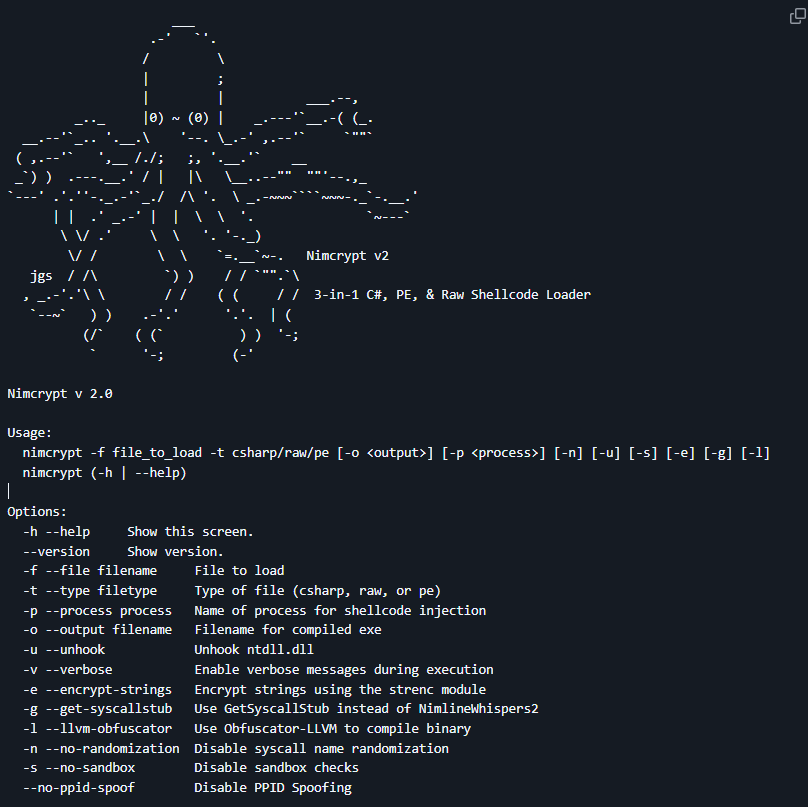
\includegraphics[width=1\textwidth]{Praxisarbeit/IMG/bilder/Nimcrypt2/nimcrypt2.png}
\caption{Nimcrypt Syntax}
\label{Nimcrypt Syntax}
\end{figure}
Zu den implementierten Funktionalitäten gehören unter anderem: die Ausführung von Shellcode über \texttt{NtQueueApcThread} (inkl. PPID-Spoofing und Mechanismen zum Blockieren Dritter DLLs), Unterstützung für Syscall-Nutzung mittels \texttt{NimlineWhispers2} und \texttt{GetSyscallStub}, Randomisierung von Syscall-Namen sowie die Fähigkeit, sowohl \texttt{.NET}-Assemblies als auch native PE-Dateien zu laden. Zur Vertraulichkeit und Verschleierung bietet das Tool AES-Verschlüsselung mit dynamischer Schlüsselerzeugung, String-Verschlüsselung sowie Kompatibilität zu LLVM-Obfuskatoren; ferner sind verschiedene Sandbox-Evasion-Mechanismen implementiert. In Praxis-Szenarien, die DLL-Injection erfordern, ist häufig die Ergänzung eines spezifischen Loaders nötig, dessen Implementierung liegt außerhalb des Rahmens dieser Arbeit, wobei festgehalten werden kann, dass Nimcrypt2 grundsätzlich die Ausführung von DLLs unterstützt.\cite{nimcrypt2}.
  \item \textbf{Veil}:  
  Veil ist ein Framework, das aus zwei Hauptmodulen besteht: einem Modul zur Erzeugung obfuskierter Payloads zur Evasion sowie einem weiteren Modul für sogenannte Ordnance-Payloads.
  \begin{figure}[H]
    \centering
    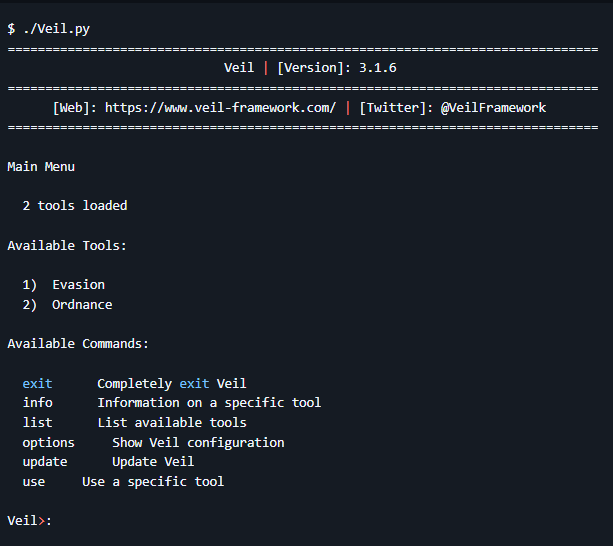
\includegraphics[width=1\textwidth]{Praxisarbeit/IMG/bilder/Veil Framework/veil1.png}
    \caption{Veil Tool}
    \label{Veil Tool}
\end{figure}
 Es dient als eine Art Bibliothek, aus der je nach Betriebssystem, gewünschter Shell-Art und Funktionsumfang die passende Payload ausgewählt werden kann. Da es sich jedoch um ein älteres Projekt handelt, werden die meisten Payloads bereits durch moderne Antivirenlösungen identifiziert und blockiert, bevor eine Ausführung erfolgen kann \cite{veil}.
  \begin{figure}[H]
    \centering
    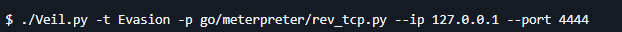
\includegraphics[width=1\textwidth]{Praxisarbeit/IMG/bilder/Veil Framework/veil2.png}
    \caption{Veil Beispiel Syntax}
    \label{Veil Beispiel Syntax}
\end{figure}
\end{enumerate}
\subsection{Durchführung und Ergebnisse}
Um einen standardisierten Testdurchlauf zu gewährleisten, wurde ein identischer Payload durch alle Obfuskationstools verarbeitet. Dieser Payload war so konzipiert, dass er bei korrekter Ausführung eine Reverse-Shell-Verbindung zur Angreifer-Maschine herstellt, wodurch ein realistisches Angriffsszenario simuliert wurde. Der Payload wurde mit \texttt{msfvenom} generiert und gehört zu den typischen Signaturen, die von modernen Sicherheitssystemen in der Regel unmittelbar erkannt werden. Dies stellte die Wirksamkeit der getesteten Tools auf eine besonders anspruchsvolle Probe.
\begin{figure}[H]
    \centering
    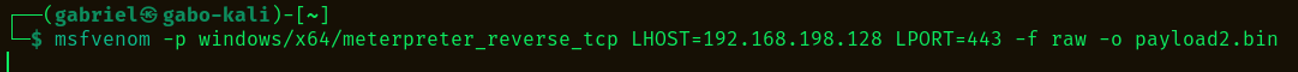
\includegraphics[width=0.8\textwidth]{Praxisarbeit/IMG/bilder/payload.png}
    \caption{Generierung des Payloads mit \texttt{msfvenom}}
    \label{fig:msfvenom}
\end{figure}
Die Durchführung begann mit der Übertragung der obfuskierten Dateien auf die Zielmaschine mit Windows-Betriebssystem. Hierfür wurde ein einfacher Webserver auf der Kali-Maschine eingerichtet, der mithilfe von Python innerhalb des Verzeichnisses mit den jeweiligen, pro Tool erzeugten Payloads betrieben wurde. Über den Webbrowser der Windows-VM konnten die Dateien anschließend heruntergeladen werden.
\begin{figure}[H]
    \centering  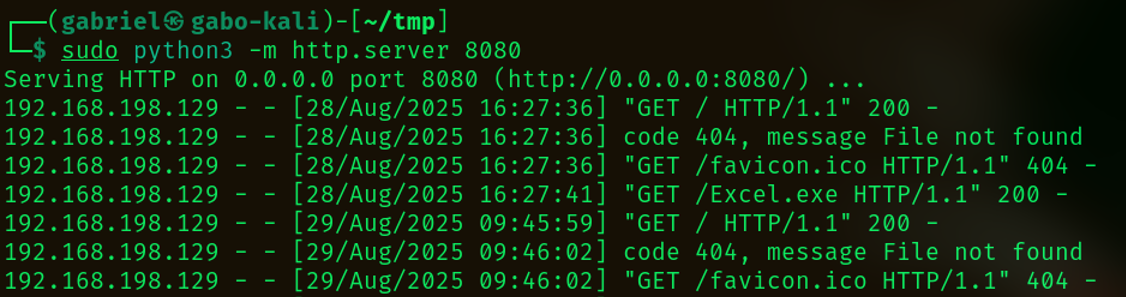
\includegraphics[width=0.8\textwidth]{Praxisarbeit/IMG/bilder/server.png}
    \caption{Aufbau des Webservers und Zugriff über den Browser}
    \label{fig:webserver}
\end{figure}
\begin{figure}[H]
    \centering  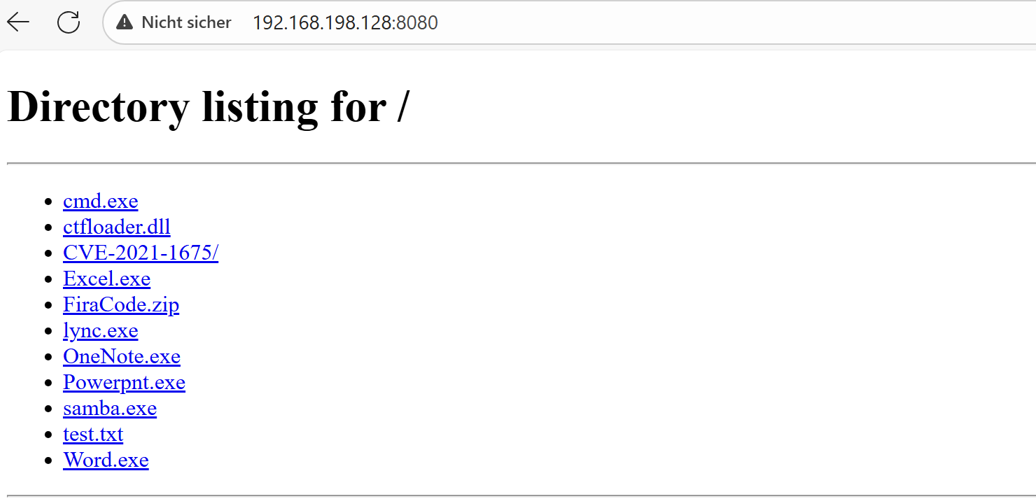
\includegraphics[width=0.8\textwidth]{Praxisarbeit/IMG/bilder/webbrowser.png}
    \caption{Aufbau des Webservers und Zugriff über den Browser}
    \label{fig:webserver}
\end{figure}
Bereits in dieser Phase zeigte sich, dass \texttt{.dll}-Dateien deutlich effektiver waren als \texttt{.exe}-Dateien, da sie vom eingesetzten EDR-System (Endpoint Detection and Response) nicht erkannt wurden. Tools, die keine \texttt{.dll}-Dateien erzeugen konnten, waren daher im Nachteil.
Das einzige Tool, das das EDR-System erfolgreich umgehen konnte, war \textbf{CTFPacker}. Es generierte eine \texttt{.dll}-Datei, die mithilfe von \texttt{rundll32} auf dem Windows-System ausgeführt wurde. Dies führte zu einer erfolgreichen Reverse-Shell-Verbindung auf der Kali-Angriffsmaschine, womit die vollständige Funktionsfähigkeit des Payloads nachgewiesen werden konnte.
\begin{figure}[H]
    \centering
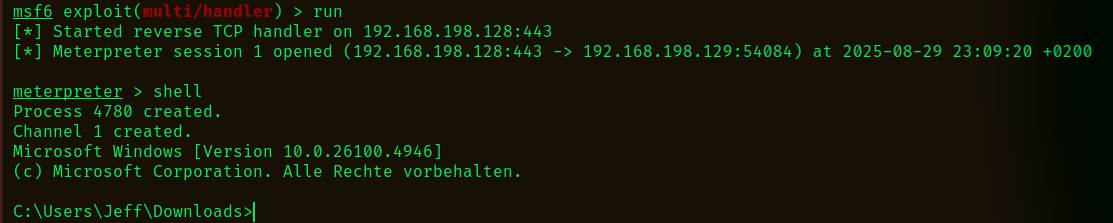
\includegraphics[width=0.8\textwidth]{Praxisarbeit/IMG/bilder/ReverseShell.png}
    \caption{Nachweis der erfolgreichen Reverse-Shell-Verbindung}
    \label{fig:reverse_shell}
\end{figure}
\newpage
\subsection{Fazit des zweiten Praxiseinsatzes und Ausblick}
Die durchgeführte Untersuchung hat gezeigt, dass Obfuskationstechniken in Penetrationstests ein essenzielles Mittel darstellen, um die Wirksamkeit moderner Sicherheitslösungen wie Antivirenprogramme und EDR-Systeme zu evaluieren. Im Rahmen der praxisnahen Tests konnte insbesondere die Erstellung und Ausführung von DLL-Payloads einen entscheidenden Vorteil hinsichtlich der Umgehung von Schutzmechanismen bieten. Dabei hat sich gezeigt, dass nicht alle Open-Source-Tools gleichwertig leistungsfähig sind: Während CTFPacker erfolgreich eine Reverse-Shell etablieren konnte, wiesen andere Werkzeuge wie ScareCrow, Donut oder Veil Einschränkungen bei der Generierung funktionaler DLLs auf oder wurden von den Sicherheitslösungen bereits vor der Ausführung erkannt.\newline
Die Ergebnisse verdeutlichen, dass die Effektivität von Verschleierungstechniken stark von der Art der generierten Payload, den eingesetzten Obfuskationsmethoden und der Kompatibilität mit aktuellen EDR-Systemen abhängt. Insbesondere die Fähigkeit, funktionsfähige DLL-Dateien zu erzeugen, stellt einen wesentlichen Erfolgsfaktor dar. Darüber hinaus wurde deutlich, dass Performance, Stabilität und Benutzerfreundlichkeit der Werkzeuge maßgeblich die Praxistauglichkeit beeinflussen.\newline
Für zukünftige Arbeiten bietet sich ein erweitertes Testdesign an, das eine größere Vielfalt an Payload-Typen, zusätzlichen Obfuskationsmethoden und realistischeren Testumgebungen umfasst. Weiterführend können dynamische Analyseverfahren kombiniert mit automatisierten Retesting-Prozessen entwickelt werden, um die langfristige Effektivität von Verschleierungstechniken systematisch zu evaluieren. Darüber hinaus eröffnet die Identifikation von Schwachstellen in aktuellen Open-Source-Tools Möglichkeiten zur Entwicklung eigener, optimierter Werkzeuge, die speziell auf moderne Sicherheitsmechanismen zugeschnitten sind. Ziel ist es, die Erkenntnisse aus dieser Arbeit nicht nur für die Qualitätssicherung von Penetrationstests zu nutzen, sondern auch Impulse für die Weiterentwicklung von Obfuskationstechniken und Evasion-Strategien zu liefern.
\newpage